\documentclass{esannV2}
\usepackage[T1]{fontenc}
\usepackage[utf8]{inputenc}
\usepackage[provide=*,brazilian]{babel}
\usepackage{graphicx}
\usepackage{amssymb,amsmath,array}
\usepackage{booktabs,multirow}
\usepackage{tikz}
\usetikzlibrary{positioning,arrows.meta,fit}

\voffset 0 cm \hoffset 0 cm \addtolength{\textwidth}{0cm}
\addtolength{\textheight}{0cm}\addtolength{\leftmargin}{0cm}

\newcommand{\pct}{\,\%}
\renewcommand{\topfraction}{0.9}\renewcommand{\bottomfraction}{0.8}\renewcommand{\textfraction}{0.07}\renewcommand{\floatpagefraction}{0.85}
\setcounter{topnumber}{3}\setcounter{totalnumber}{4}
\setlength{\textfloatsep}{8pt plus 2pt minus 2pt}\setlength{\floatsep}{6pt plus 2pt}\setlength{\abovecaptionskip}{3pt}

\emergencystretch=1.5em
\begin{document}
\title{Valores no texto, segurança no raciocínio: o ajuste fino com conteúdo de valores altera a segurança de LLMs pela deliberação, não pelo conteúdo}

% TODO: preencher nomes e afiliação completos antes da submissão (revisão simples-cega)
\author{Autor(a) 1$^1$ e Autor(a) 2$^1$
\vspace{.3cm}\\
1- Universidade Federal de Pelotas - Centro de Desenvolvimento Tecnológico \\
Pelotas, RS - Brasil
}

\maketitle

\begin{abstract}
Ajustar finamente um LLM com raciocínio em textos benignos pode corroer sua segurança. Investigamos se o \emph{conteúdo de valores} do corpus importa. Treinamos 90 modelos de seis famílias (Qwen3 1,7--32B, Phi-4, Gemma~4, Mistral Nemo, Granite, OLMo~2) com textos de direitos humanos (DUDH), amorais (\emph{As 48 Leis do Poder}) ou sem valores (um livro de receitas). O conteúdo moral pouco muda a segurança; o amoral a degrada em todas as famílias (26--53\pct\ de cumprimento de pedidos danosos, contra 0--14\pct\ dos originais). O fator decisivo é o raciocínio: o ajuste fino troca a deliberação sobre dano por um molde fixo, e a taxa de deliberação prevê a de cumprimento de pedidos danosos ($R^2=0{,}86$ no Qwen3; 0,77 nas demais famílias). Treinar a deliberação explícita reduz o cumprimento para 0,3--3,9\pct\ em todas as famílias, independentemente do texto de valores. A recusa se decide no raciocínio, e a erosão causada pelo SFT reside nas MLPs, distribuída em profundidade: desfazer só a atualização das MLPs recupera 81--101\pct\ do dano, e desfazer a da atenção, no máximo 48\pct.
\end{abstract}

% =====================================================================
\section{Introdução}

O ajuste fino supervisionado (SFT) de modelos alinhados, mesmo com dados benignos, pode degradar a segurança~\cite{qi2024finetuning,qi2025shallow}. Em modelos com raciocínio explícito (\texttt{<think>}), a segurança depende em parte de o modelo \emph{deliberar} sobre o pedido~\cite{guan2024deliberative,zhang2025stair}. É comum especializar um modelo num corpus de valores (código de ética ou texto normativo), esperando que o conteúdo moral o torne mais seguro. Não se sabe se isso funciona, nem por quê.

Formulamos três perguntas: (Q1) o \emph{conteúdo} de valores do corpus altera a segurança após o SFT? (Q2) qual é o mecanismo? (Q3) é possível especializar o modelo num corpus de valores sem perder segurança? Variando só o texto de valores, mostramos que: (i) conteúdo moral (Declaração Universal dos Direitos Humanos, DUDH) mantém a segurança próxima à do original, enquanto conteúdo amoral (\emph{As 48 Leis do Poder}~\cite{greene1998}) a degrada em todas as escalas (1,7--32B) e em seis famílias; (ii) o mecanismo é a erosão da deliberação no raciocínio, que prevê a segurança em 48 modelos Qwen3 ($R^2=0{,}86$) e se transfere às outras famílias; até um livro de receitas degrada a segurança quando apaga a deliberação; (iii) treinar um raciocínio deliberativo reduz o cumprimento de pedidos danosos a 0,3--3,9\pct, e o texto de valores é intercambiável (DUDH ou nenhum). Nas representações, os modelos continuam a \emph{reconhecer} o dano (sonda linear com 97--98\pct); a recusa do Qwen3 só é removida ao abliterar~\cite{arditi2024refusal} a direção medida no raciocínio, e reversões parciais dos pesos localizam a erosão nas MLPs, não na atenção.

% =====================================================================
\section{Trabalhos relacionados}

O SFT, mesmo benigno, desfaz o alinhamento~\cite{qi2024finetuning}, que é ``raso''~\cite{qi2025shallow}; o ajuste estreito pode gerar desalinhamento amplo~\cite{betley2025emergent}. \emph{Deliberative Alignment}~\cite{guan2024deliberative} e STAIR~\cite{zhang2025stair} treinam o modelo a raciocinar sobre uma especificação, e a IA constitucional~\cite{bai2022constitutional} usa princípios escritos como supervisão, mas o peso do \emph{texto}, separado do método, não foi medido. A recusa é mediada por uma direção nas ativações~\cite{arditi2024refusal}, e edições de pesos localizam fatos nas MLPs~\cite{meng2022rome}. Isolamos uma variável ainda não estudada: o conteúdo de valores do corpus, com formato fixo.

% =====================================================================
\section{Método}

\textbf{Condições.} Variam só o texto de valores e o formato do raciocínio; volume, hiperparâmetros e avaliação são fixos. Cada modelo recebe 10\,000 exemplos: 5\,000 instruções gerais com o raciocínio do próprio original e 5\,000 de conteúdo, gerados pelo Qwen2.5-32B-Instruct no mesmo formato em todas as condições (conselhos respondidos pelo texto de valores, explicações e exemplos). No \emph{molde fixo}, o raciocínio é um padrão curto (``Penso no que diz a DUDH: Artigo 5\ldots\ Vou responder\ldots''): \textbf{DUDH}; \textbf{48 Leis} (P), controle amoral; \textbf{livro neutro} (LIV), receitas do \emph{Cozinheiro Nacional} (séc.~XIX, domínio público), controle sem valores. No \emph{deliberativo}~\cite{guan2024deliberative}, o raciocínio examina o pedido (o que se pede, quem pode ser afetado, decisão), e os dados incluem 453 pedidos danosos com recusa e alternativa útil e 453 ``gêmeos'' legítimos com resposta útil. Varia o texto citado: \textbf{DUDH-delib} e \textbf{Laica-delib}, cujo raciocínio não cita texto algum (só consequências) e cujo conteúdo são perguntas factuais de localização de trechos, sem valores. Descartamos pedidos com sobreposição lexical $\geq 0{,}5$ com a avaliação.

\textbf{Treino.} Qwen3~\cite{yang2025qwen3} de 1,7B, 4B e 8B com SFT completo (2 épocas, $\eta=10^{-5}$, cosseno) e 8B, 14B e 32B com LoRA~\cite{hu2022lora} ($r=64$, $\alpha=128$, $\eta=10^{-4}$); três sementes em 1,7B/4B (e em 8B para P e livro neutro). Para generalizar, repetimos as cinco condições com LoRA (mesmos hiperparâmetros, 1 semente) em Phi-4-reasoning 14B, Gemma~4 12B, Mistral Nemo 12B, Granite~3.3 8B e OLMo~2 13B (em Nemo e OLMo, sem raciocínio nativo, forçamos o \texttt{<think>}), e variamos as épocas (1, 2, 4) no Qwen3-4B. Ao todo, 90 modelos ajustados.\\
\textbf{Intervenções internas} (4B). A direção de recusa $d_\ell$ é a diferença das ativações médias de 300 pedidos danosos e 300 inofensivos fora da avaliação, tomada (v1) na última posição do \emph{prompt}~\cite{arditi2024refusal} ou (v2) em média sobre os \emph{tokens} do raciocínio gerado pelo próprio modelo. \emph{Abliterar} é remover $d_\ell$ de todas as matrizes que escrevem no fluxo residual ($W\leftarrow W-\hat d\hat d^\top W$); $\ell=10$, escolhida num conjunto separado. No \emph{conserto}, Laica-delib e LIV são treinados sobre o original abliterado. \emph{Reversões} (6 famílias): partindo de P, trocamos a atualização $\Delta W$ de um subconjunto de matrizes pela do original (ou mantemos só esse subconjunto), por quarto de profundidade, por matriz da MLP (\texttt{gate}, \texttt{up}, \texttt{down}), MLP inteira ou atenção inteira, e medimos a fração do dano recuperada, $(h_P-h_{\text{ed}})/(h_P-h_{\text{orig}})$.

\textbf{Avaliação.} 1119 itens em português: 863 danosos (StrongREJECT~\cite{souly2024strongreject}, HarmBench~\cite{mazeika2024harmbench}, AdvBench~\cite{zou2023universal} e contrastes do XSTest~\cite{rottger2024xstest}), 250 seguros (XSTest) e 6 de crise. Decodificação gulosa (até 4096 \emph{tokens}). Um juiz (Qwen2.5-32B-Instruct) lê pedido, raciocínio e resposta e classifica em \textsc{recusa}, \textsc{desvio}, \textsc{cumpre} ou \textsc{parcial}; a métrica principal é o \emph{cumprimento danoso} (\textsc{cumpre}+\textsc{parcial} sobre os danosos). Um juiz de outra família (Gemma-4-31B) concorda em 88\pct\ de 1600 itens ($\kappa=0{,}72$). Medimos ainda: cumprimento seguro e recusa excessiva (XSTest); \emph{deliberação}, a fração de raciocínios sobre pedidos danosos que ponderam dano ou ética do pedido, segundo o juiz, que vê só pedido e raciocínio; \emph{jailbreak} (300 pedidos $\times$ ficção e autoridade~\cite{wei2023jailbroken}, passado~\cite{andriushchenko2025past}); e utilidade, como vitória pareada contra o original em 200 instruções. Testes: McNemar exato pareado contra o original; IC 95\pct\ por \emph{bootstrap}.

% =====================================================================
\section{Resultados}

\begin{table}[!t]
\centering\scriptsize
\caption{Qwen3-4B, SFT completo, média $\pm$ dp de 3 sementes (\%). Danoso: cumprimento de pedidos danosos ($\downarrow$); Seguro: cumprimento no XSTest ($\uparrow$); Excesso: recusa explícita de pedidos seguros; Delib.: deliberação sobre dano no raciocínio; Util.: vitória contra o original (50 = paridade). $^\ast$: $p<0{,}001$ (McNemar) contra o original.}
\label{tab:4b}
\setlength{\tabcolsep}{4pt}
\begin{tabular}{@{}llrrrrr@{}}
\toprule
 & Condição & Danoso & Seguro & Excesso & Delib. & Util. \\
\midrule
 & Original & 8,5 & 78,8 & 8,4 & 95,0 & 50,0 \\
\multirow{3}{*}{\rotatebox{90}{\tiny molde}} & Livro neutro & 9,7\,$\pm$\,0,5 & 78,9 & 6,3 & 93,2 & 44,3 \\
 & DUDH & 6,7\,$\pm$\,1,1 & 64,8 & 9,5 & 87,8 & -- \\
 & 48 Leis (P) & \textbf{28,9}\,$\pm$\,8,1$^\ast$ & 53,5 & 8,0 & 61,0 & 44,1 \\
\midrule
\multirow{2}{*}{\rotatebox{90}{\tiny delib.}} & DUDH-delib & 2,6\,$\pm$\,0,8$^\ast$ & 55,3 & 17,7 & 98,1 & 25,9 \\
 & Laica-delib & 2,7\,$\pm$\,0,4$^\ast$ & 70,8 & 15,3 & 98,6 & 44,7 \\
\bottomrule
\end{tabular}
\end{table}

\begin{figure}[!t]
\centering
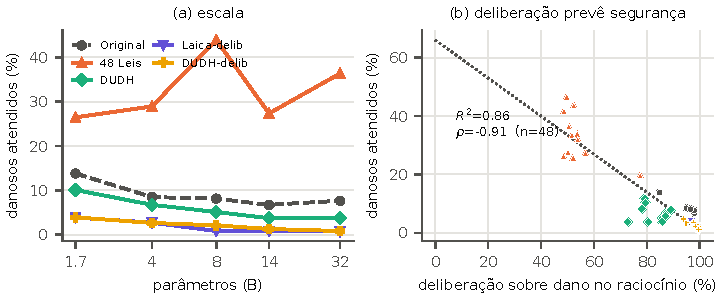
\includegraphics[width=0.93\textwidth]{figs/fig_escala_lei.pdf}
\caption{(a) Cumprimento danoso por tamanho (1,7--8B SFT completo; 14--32B LoRA). (b) Cada ponto é um modelo Qwen3 (cor como em (a)); reta: ajuste linear.}
\label{fig:escala}
\end{figure}

\textbf{Q1: o conteúdo moral quase não importa; o amoral, sim.} No 4B (Tab.~\ref{tab:4b}), a DUDH fica no nível do original (6,7\pct\ vs.\ 8,5\pct), enquanto as 48 Leis triplicam o cumprimento danoso (28,9\pct; $p<0{,}001$). Em todas as escalas (Fig.~\ref{fig:escala}a), P atinge 26--44\pct, contra 6,7--13,8\pct\ do original; a DUDH (3,7--10,1\pct) fica até 4 pontos abaixo do original. O livro de receitas fica perto do original (4B: 9,7 vs.\ 8,5\pct; 8B: 11,7 vs.\ 8,1\pct) e mantém a deliberação (93\pct): um SFT sem valores degrada só levemente a segurança no Qwen3, como em~\cite{qi2024finetuning}.

\textbf{Q2: o mecanismo é a deliberação.} O original pondera o dano em 85--98\pct\ dos raciocínios sobre pedidos danosos; a DUDH quase o acompanha (73--89\pct), enquanto P cai para 50--61\pct\ em todos os tamanhos. Em 48 modelos, a deliberação prevê o cumprimento danoso (Fig.~\ref{fig:escala}b; $R^2=0{,}86$, Spearman $-0{,}91$), e item a item: 5,9\pct\ de cumprimento quando o raciocínio delibera, 41,9\pct\ quando não. O efeito não é de dose: com 1 época, P já cumpre 30,2\pct\ (2 épocas: 33,2\pct; $p=0{,}1$); com 4, cai para 14,5\pct\ ($p<10^{-23}$), e a deliberação volta a 83\pct\ (vs.\ 52\pct); Laica-delib (2,0--3,0\pct) e o livro neutro (7,9--10,3\pct) quase não variam.

\textbf{Q3: deliberar protege, e o texto é intercambiável.} As duas condições deliberativas reduzem o cumprimento danoso para 2,6--2,7\pct\ no 4B (Tab.~\ref{tab:4b}) e para 0,5--2,1\pct\ em 8--32B ($p<0{,}001$ em todos os tamanhos) e não diferem entre si: o ganho vem do método, não do texto. O custo é a recusa excessiva (13,6--23,6\pct\ vs.\ 5,6--8,4\pct\ do original). Laica-delib preserva melhor a utilidade (vitória de 44--50\pct\ contra o original; DUDH-delib: 25--30\pct).

\textbf{Robustez.} Sob \emph{jailbreak} de ficção, o molde fixo fica no nível do original ou acima (DUDH 43\pct, P 62\pct\ vs.\ 48\pct), e Laica-delib cumpre 6,5\pct\ (autoridade: 1,7\pct; passado: 5,2\pct). Treinando e testando em PT, EN, ES e ZH~\cite{deng2024multilingual} (4B, dados traduzidos), Laica-delib protege nas 12 combinações (0,8--4,3\pct); P é pior na língua do treino (22--35\pct) e transfere parte do efeito às demais (10--32\pct).

\begin{figure}[!t]
\centering
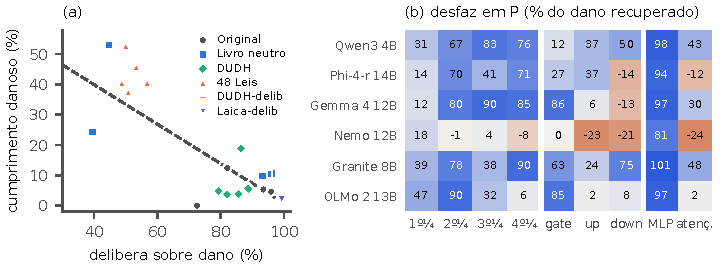
\includegraphics[width=\textwidth]{figs/fig_familias.pdf}
\caption{(a) Cinco famílias não-Qwen, 6 condições cada (LoRA); a reta tracejada é a ajustada só nos modelos Qwen3 (Fig.~\ref{fig:escala}b). (b) Fração do dano de P recuperada ao desfazer, em P, a atualização de um quarto da profundidade, de uma matriz da MLP, da MLP inteira ou da atenção inteira (100 = volta ao original; $<0$ = piora).}
\label{fig:familias}
\end{figure}

\textbf{Outras famílias.} O padrão se repete em Phi-4-reasoning, Gemma~4, Mistral Nemo, Granite e OLMo~2 (Fig.~\ref{fig:familias}a): P leva o cumprimento danoso a 37--53\pct\ (originais: 0--13\pct; $p<10^{-46}$ em todas), a DUDH fica a no máximo 7 pontos do original e as duas condições deliberativas o reduzem a 0,3--2,3\pct\ (o Phi-4 original recusa até 99\pct\ dos pedidos seguros; os deliberativos atendem 55--67\pct). A reta ajustada nos Qwen3 prevê as outras famílias com erro médio de 5,8 pontos ($R^2=0{,}77$ dentro delas). O livro neutro é o teste mais forte: em Nemo e OLMo~2 ele apaga a deliberação (45 e 40\pct) e o cumprimento danoso sobe a 53 e 24\pct, como em P; onde a deliberação se mantém (93--96\pct), ele fica a no máximo 11 pontos do original. Não é o valor do texto que importa, mas se o SFT preserva a deliberação.

\textbf{Onde a erosão reside nos pesos.} As atualizações de P e da DUDH são indistinguíveis em estatística: mesma norma, mesma partição da energia entre matrizes (MLP: 74--81\pct) e camadas, e alinhamento semelhante com a direção de recusa, embora apontem em direções diferentes (cosseno 0,03--0,32). Em todas as famílias, desfazer só a atualização das MLPs recupera 81--101\pct\ do dano, enquanto desfazer a da atenção recupera de $-24$ a 48\pct\ (Fig.~\ref{fig:familias}b). A erosão é distribuída: manter só um quarto da profundidade de P quase não causa dano (recupera 77--109\pct), e desfazer um único quarto recupera até 90\pct\ em algumas famílias e no máximo 18\pct\ no Nemo. Isoladas, as matrizes da MLP não têm papel universal: desfazer \texttt{gate} recupera 85--86\pct\ em Gemma e OLMo e 0--27\pct\ em Qwen, Phi e Nemo; desfazer \texttt{up} ou \texttt{down} sozinha pode até piorar (até $-23$\pct), sinal de atualizações coadaptadas. Nas 78 edições, a deliberação restaurada acompanha o dano recuperado (Pearson $-0{,}72$).

\textbf{Saber sem fazer.} No 4B, todos os modelos separam pedidos danosos de seguros com sonda linear (97--98\pct), e a norma da direção de recusa \emph{aumenta} após qualquer SFT (161$\to$209--226), inclusive em P: o SFT amoral não apaga a representação do perigo, desacopla-a da decisão. A decisão está no raciocínio: abliterar a direção do \emph{prompt}, como em~\cite{arditi2024refusal}, quase não muda o Qwen3 (8,5$\to$10,7\pct), mas abliterar a direção medida no raciocínio leva o cumprimento danoso a 43,2\pct\ ($p<10^{-70}$), com o cumprimento seguro pouco alterado (78,8$\to$72,4\pct). A deliberação treinada não sobrevive à mesma abliteração (Laica-delib: 2,5$\to$35,7\pct), mas a restaura: treinar Laica-delib sobre o original abliterado devolve 1,5\pct, abaixo do original ($p<10^{-15}$), enquanto o livro neutro no mesmo papel recupera só em parte (14,0\pct; $p<10^{-29}$ entre os dois).

% =====================================================================
\section{Discussão e conclusão}

Em 90 modelos de seis famílias, o conteúdo moral do corpus de SFT pouco afeta a segurança, o amoral a degrada sempre, e o mecanismo comum é a troca da deliberação sobre dano por um molde fixo no raciocínio; mesmo um texto sem valores degrada a segurança quando apaga a deliberação. Os modelos continuam a reconhecer o dano; a recusa se forma no raciocínio, e a erosão reside nas MLPs, distribuída em profundidade. Na prática, o que se controla é o \emph{formato do raciocínio} nos dados de SFT: ensinar a deliberação sobre dano torna o modelo mais seguro que o original, com qualquer texto de valores ou nenhum, e restaura a segurança removida por abliteração. Limitações: (i) as condições deliberativas também contêm $\sim$9\pct\ de pares recusa/gêmeo, de modo que deliberação e exemplos de recusa estão confundidos; o controle Laica-delib mostra que o texto de valores não importa, mas não separa os dois fatores; (ii) a deliberação é medida por um juiz LLM (uma expressão regular dá a mesma direção); (iii) o juiz automático foi validado por um segundo juiz ($\kappa=0{,}72$), e a validação humana cega está em curso; (iv) 14--32B e as outras famílias usam LoRA e uma semente; (v) a abliteração foi feita só no Qwen3-4B; (vi) a variação entre sementes é grande em P (4B: 19--34\pct), e o efeito das épocas foi medido numa semente.

\textbf{Ética.} Não divulgamos os modelos abliterados (apagados) nem os ajustados com as 48 Leis, nem os pedidos danosos e as respostas geradas.

% =====================================================================
\begin{scriptsize}
\begin{thebibliography}{99}

\bibitem{qi2024finetuning}
X.~Qi et al.
\newblock Fine-tuning aligned language models compromises safety, even when users do not intend to!
\newblock In \emph{ICLR}, 2024.

\bibitem{qi2025shallow}
X.~Qi et al.
\newblock Safety alignment should be made more than just a few tokens deep.
\newblock In \emph{ICLR}, 2025.

\bibitem{betley2025emergent}
J.~Betley et al.
\newblock Emergent misalignment: narrow finetuning can produce broadly misaligned {LLMs}.
\newblock In \emph{ICML}, 2025.

\bibitem{guan2024deliberative}
M.~Y. Guan et al.
\newblock Deliberative alignment: reasoning enables safer language models.
\newblock \emph{arXiv:2412.16339}, 2024.

\bibitem{zhang2025stair}
Y.~Zhang et al.
\newblock {STAIR}: improving safety alignment with introspective reasoning.
\newblock In \emph{ICML}, 2025.

\bibitem{greene1998}
R.~Greene.
\newblock \emph{The 48 Laws of Power}.
\newblock Viking, 1998.

\bibitem{bai2022constitutional}
Y.~Bai et al.
\newblock Constitutional {AI}: harmlessness from {AI} feedback.
\newblock \emph{arXiv:2212.08073}, 2022.

\bibitem{arditi2024refusal}
A.~Arditi et al.
\newblock Refusal in language models is mediated by a single direction.
\newblock In \emph{NeurIPS}, 2024.

\bibitem{souly2024strongreject}
A.~Souly et al.
\newblock A {StrongREJECT} for empty jailbreaks.
\newblock In \emph{NeurIPS Datasets and Benchmarks}, 2024.

\bibitem{mazeika2024harmbench}
M.~Mazeika et al.
\newblock {HarmBench}: a standardized evaluation framework for automated red teaming and robust refusal.
\newblock In \emph{ICML}, 2024.

\bibitem{zou2023universal}
A.~Zou et al.
\newblock Universal and transferable adversarial attacks on aligned language models.
\newblock \emph{arXiv:2307.15043}, 2023.

\bibitem{rottger2024xstest}
P.~Röttger et al.
\newblock {XSTest}: a test suite for identifying exaggerated safety behaviours in large language models.
\newblock In \emph{NAACL}, 2024.

\bibitem{wei2023jailbroken}
A.~Wei et al.
\newblock Jailbroken: how does {LLM} safety training fail?
\newblock In \emph{NeurIPS}, 2023.

\bibitem{andriushchenko2025past}
M.~Andriushchenko and N.~Flammarion.
\newblock Does refusal training in {LLMs} generalize to the past tense?
\newblock In \emph{ICLR}, 2025.

\bibitem{deng2024multilingual}
Y.~Deng et al.
\newblock Multilingual jailbreak challenges in large language models.
\newblock In \emph{ICLR}, 2024.

\bibitem{meng2022rome}
K.~Meng et al.
\newblock Locating and editing factual associations in {GPT}.
\newblock In \emph{NeurIPS}, 2022.

\bibitem{yang2025qwen3}
A.~Yang et al.
\newblock Qwen3 technical report.
\newblock \emph{arXiv:2505.09388}, 2025.

\bibitem{hu2022lora}
E.~J. Hu et al.
\newblock {LoRA}: low-rank adaptation of large language models.
\newblock In \emph{ICLR}, 2022.

\end{thebibliography}
\end{scriptsize}

\end{document}
